\chapter{Lab Report}
\section{Week 1 Naive Fourier Transform}
    This week comprised of performing a Fourier Transform and Inverse Fourier Transform on a .pgm image file. The original image is of a wolf shown in Figure \autoref{fig:wolf_image}

    Supporting Java classes were provided, these include Display2dFT.java, DisplayDensity.java, ReadPGM.java and SimpleFT a skeleton program to code in.

    DisplayDensity.java displays a greyscale image from a 2D array, with smaller values dark and larger values white. ReadPGM.java parses the .pgm file for use in the skeleton program and Display2dFT.java allows the Fourier Transform output to be represented graphically, using colour to represent imaginary number components.
    
    \begin{figure}[H]
        \centering
        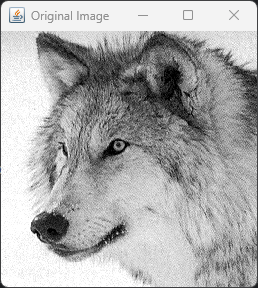
\includegraphics[width=0.8\columnwidth]{Figures/Week 1/W1-Wolf-Original.png}
        \caption{A screenshot of the original wolf image}
        \label{fig:wolf_image}
        
    \end{figure}
    
    \subsection{Discrete Fourier Transform}
    The equation shown in Figure \autoref{fig:equation-FT} needs to be implemented to perform a Discrete Fourier Transform, C is an array N, N in size.
    \vspace{15mm}


    \begin{center}
        \begin{equation}
            C_{kl} = 1/N^2 \sum_{m=0}^{N-1} \sum_{n=0}^{N-1}\ X_{mn} . e^{-2\pi i(km+nl)/N}
            \label{fig:equation-FT}
        \end{equation}  
    \end{center}

   
    \begin{figure}[H]
        \centering
        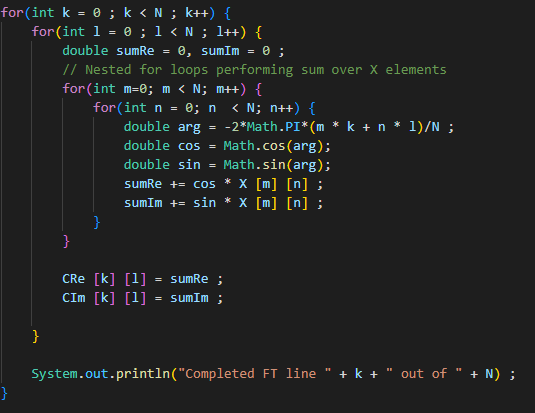
\includegraphics[width=1\columnwidth]{Figures/Week 1/W1-SimpleFT-Completed-For-Loop.png}
        \caption{A screenshot of the implementation of the Fourier Transform}
        \label{fig:wolf-FT-code}
    \end{figure}
    
    \begin{figure}[H]
        \centering
        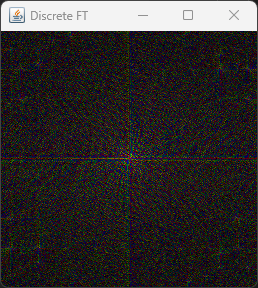
\includegraphics[width=0.8\columnwidth]{Figures/Week 1/W1-FT.png}
        \caption{A screenshot of the Discrete Fourier Transform graphical output}
        \label{fig:wolf-DFT}
    \end{figure}
    
    
    \subsection{Inverse Discrete Fourier Transform}


        \begin{center}
        \begin{equation}
            X_{mn} = \sum_{k=0}^{N-1} \sum_{l=0}^{N-1}\ C_{kl} . e^{2\pi i(km+nl)/N}
            \label{fig:equation-InverseFT}
        \end{equation}  
        \end{center}

        \begin{figure}[H]
            \centering
            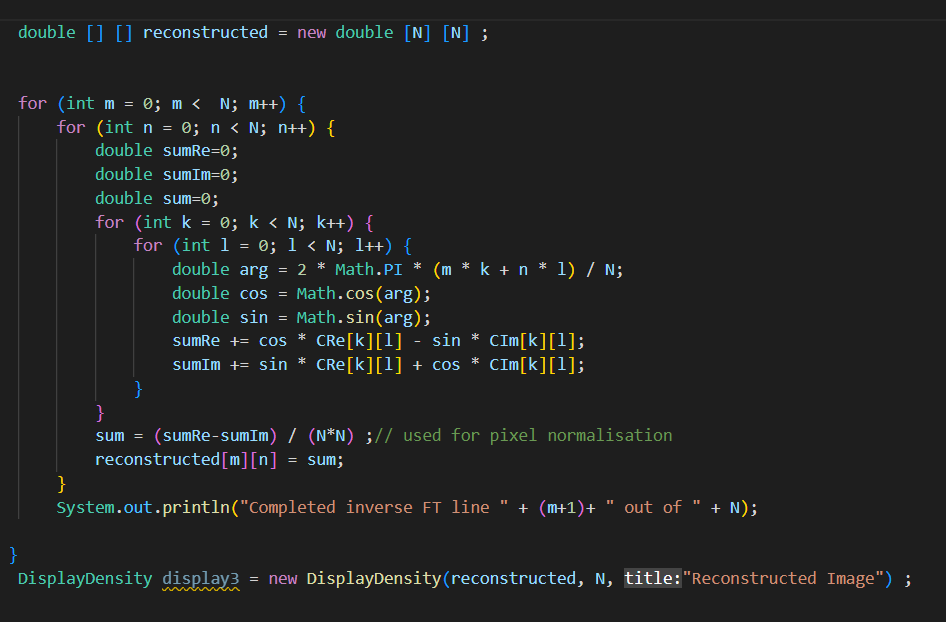
\includegraphics[width=1\columnwidth]{Figures/Week 1/W1-SimpleFT-InverseDFT-Implementation.png}
            \caption{A screenshot of the java inverse DFT implementation}
            \label{fig:inverse-DFT-Code}
    \end{figure}
    
        \begin{figure}[H]
            \centering
            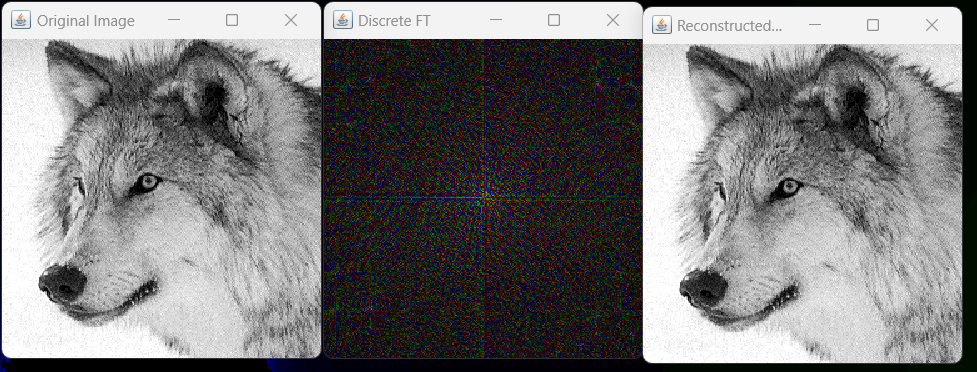
\includegraphics[width=0.8\columnwidth]{Figures/Week 1/W1-SimpleFT-InverseDFT-Graphical-Outputs.png}
            \caption{Graphical output of the program - inverse DFT reconstruction on the right side}
            \label{fig:inverse-DFT-Images-Output}
    \end{figure}
    
        \begin{figure}[H]
            \centering
            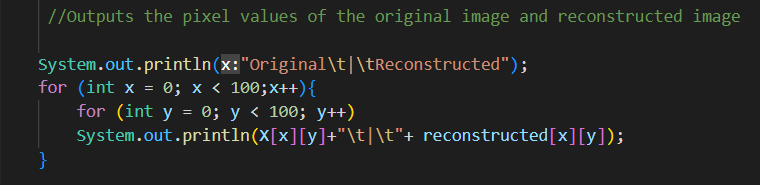
\includegraphics[width=1\columnwidth]{Figures/Week 1/W1-SimpleFT-InverseDFT-Test-1.0-code.png}
            \caption{A screenshot of the testing code}
            \label{fig:Testing-Code}
    \end{figure}
    
        \begin{figure}[H]
            \centering
            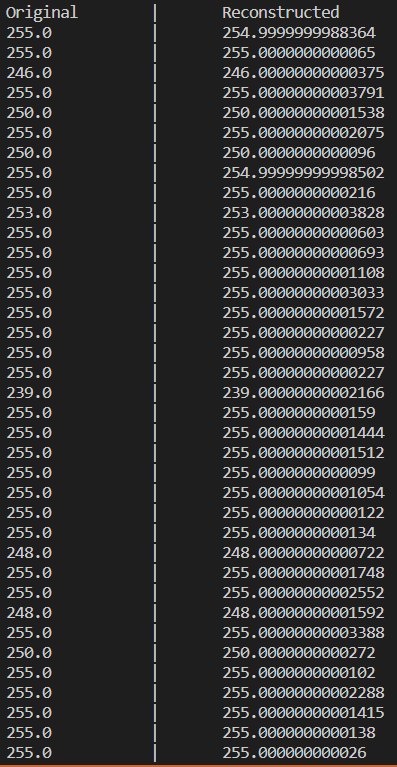
\includegraphics[width=.49\columnwidth]{Figures/Week 1/W1-SimpleFT-InverseDFT-Test-1.0-Output.png}
            \caption{A screenshot of the testing code output}
            \label{fig:Testing-Code-output}
        \end{figure}
        
        \begin{figure}[H]
            \centering
            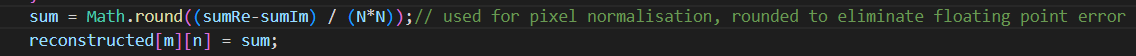
\includegraphics[width=1\columnwidth]{Figures/Week 1/W1-SimpleFT-InverseDFT-Floating-Point-Fix.png}
            \caption{A screenshot of code to fix floating point error}
            \label{fig:floating-Point-Fix}
        \end{figure}
        
    
        \begin{figure}[H]
            \centering
            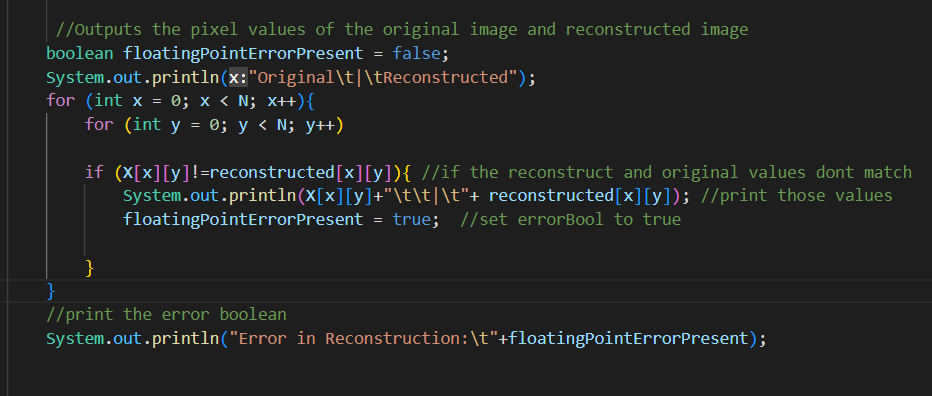
\includegraphics[width=.49\columnwidth]{Figures/Week 1/W1-SimpleFT-InverseDFT-Test-2.0-code.png}
            \caption{A screenshot of code to test the floating point error fix}
            \label{fig:floating-Point-Fixed-test}
        \end{figure}
    
        \begin{figure}[H]
            \centering
            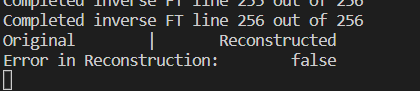
\includegraphics[width=0.8\columnwidth]{Figures/Week 1/W1-SimpleFT-InverseDFT-Test-2.0-CLI-Output.png}
            \caption{A screenshot of console output showing floating point error test has passed}
            \label{fig:floating-Point-Fixed-CLI-Output}
        \end{figure}
        
        \begin{figure}[H]
            \centering
            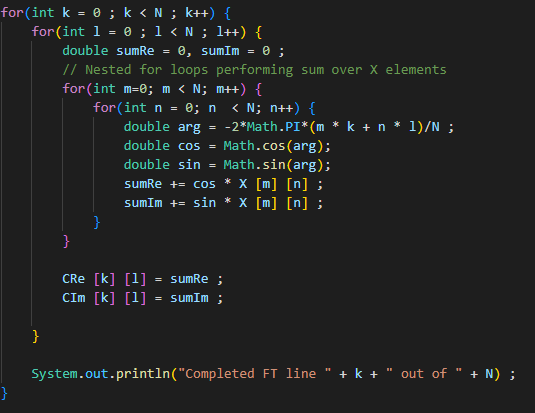
\includegraphics[width=0.8\columnwidth]{Figures/Week 1/W1-SimpleFT-Completed-For-Loop.png}
            \caption{A screenshot of graphical image reconstruction floating point error fix}
            \label{fig:floating-Point-Fixed-Graphical-Output}
        \end{figure}
    
    
    \subsection{Filtering}
   
    \subsubsection{Low Pass Filter}
          \begin{figure}[H]
        \centering
        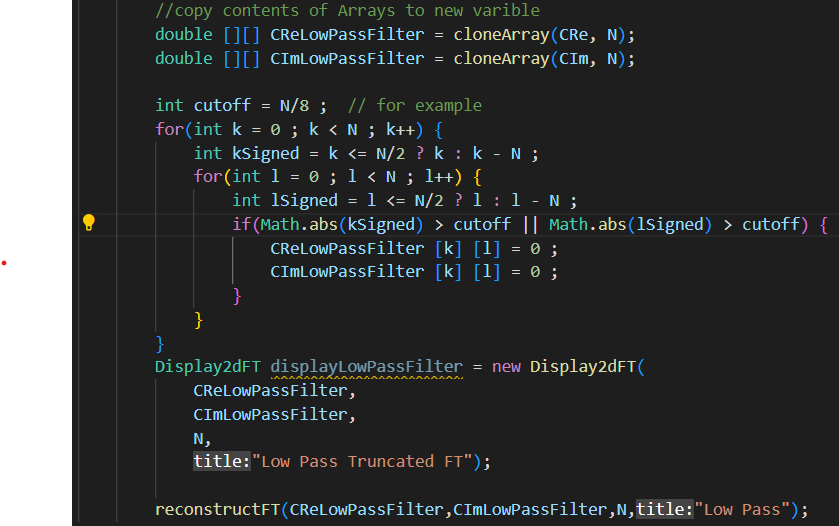
\includegraphics[width=0.8\columnwidth]{Figures/Week 1/W1-Low-Pass-Code.png}
        \caption{Screenshot of FT low pass filter code}
        \label{fig:Low-Pass-Filter-code}
      \end{figure}

      \begin{figure}[H]
        \centering
        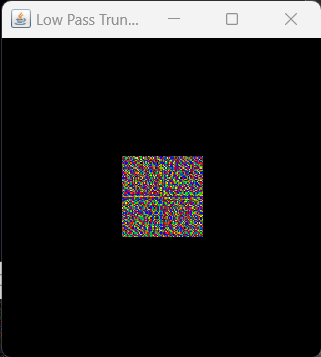
\includegraphics[width=0.8\columnwidth]{Figures/Week 1/W1-Low-Pass-Truncated.png}
        \caption{Screenshot of the low pass filter truncated FT graphical output}
        \label{fig:Low-Pass-Filter-Truncated}
      \end{figure}

      \begin{figure}[H]
        \centering
        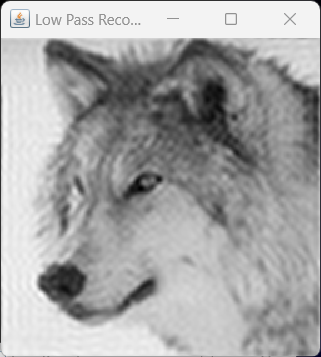
\includegraphics[width=0.8\columnwidth]{Figures/Week 1/W1-Low-Pass-Reconstructed.png}
        \caption{Screenshot of the low pass filter reconstructed image output}
        \label{fig:Low-Pass-Filter-Image}
      \end{figure}
    
    
    \subsubsection{High Pass Filter}
    
      \begin{figure}[H]
        \centering
        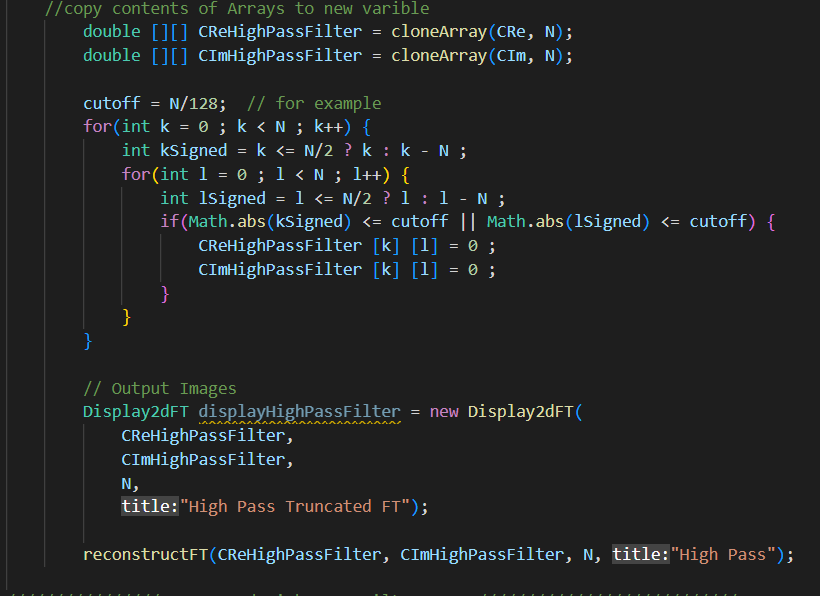
\includegraphics[width=1\columnwidth]{Figures/Week 1/W1-High-Pass-Code.png}
        \caption{Screenshot of FT high pass filter code}
        \label{fig:High-Pass-Filter-code}
      \end{figure}

      \begin{figure}[H]
        \centering
        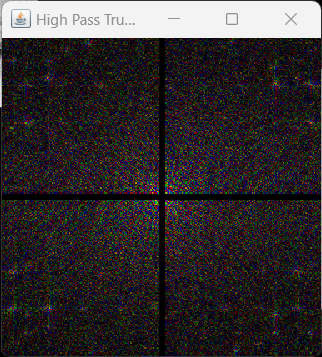
\includegraphics[width=0.8\columnwidth]{Figures/Week 1/W1-High-Pass-Truncated.png}
        \caption{Screenshot of the high pass filter truncated FT graphical output}
        \label{fig:High-Pass-Filter-Truncated}
      \end{figure}

      \begin{figure}[H]
        \centering
        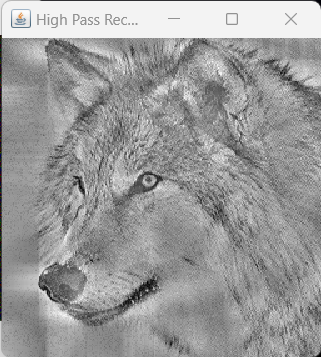
\includegraphics[width=0.8\columnwidth]{Figures/Week 1/W1-High-Pass-Reconstructed.png}
        \caption{Screenshot of the high pass filter reconstructed image output}
        \label{fig:High-Pass-Filter-Image}
      \end{figure}

      \subsubsection{Combined Filters}
        \begin{figure}[H] 
            \centering
            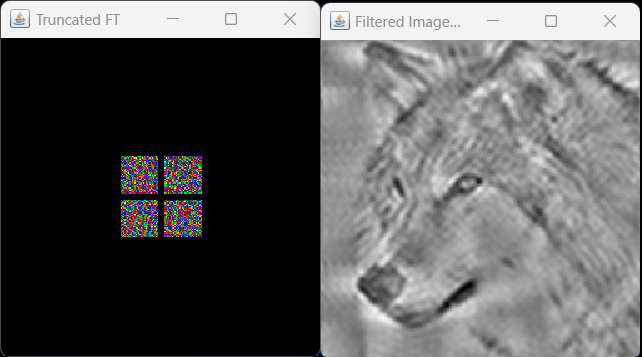
\includegraphics[width=0.8\columnwidth]{Figures/Week 1/W1-Both-Filters.png}
            \caption{Screenshot of the graphical output when filters are combined}
            \label{fig:Combined-Filters}
        \end{figure}



\section{Week 2 - Fast Fourier Transform}
This week a Fast Fourier Transform was implemented and benchmarked. Each program was run three times to compare processing speeds. 

\subsection{2D FFT Implementation}
To implement a 2D FFT using the fft1d method from the sample FFT class, a helper function was implemented to transpose the 2D arrays. This is show in \autoref{fig:transpose-code} 

    \begin{figure}[H] 
        \centering
        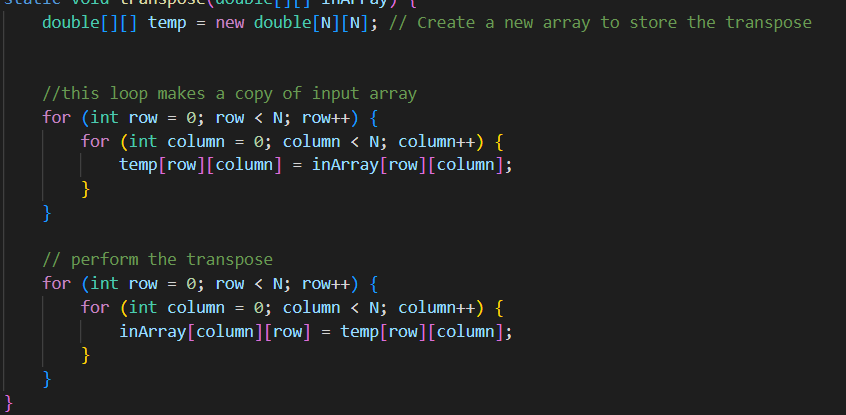
\includegraphics[width=0.8\columnwidth]{Figures/Week 2/Transpose Implementation.png}
        \caption{Screenshot of Java code showing the transpose function implementation}
        \label{fig:transpose-code}
    \end{figure}

    \begin{figure}[H] 
        \centering
        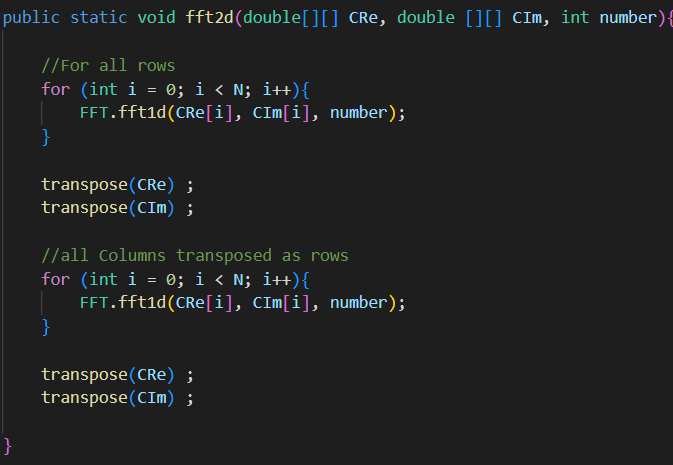
\includegraphics[width=0.8\columnwidth]{Figures/Week 2/2dFFT Implementation.png}
        \caption{Screenshot of Java code showing the 2D FFT function implementation}
        \label{fig:2dFFT-code}
    \end{figure}


\subsection{Benchmarking}
Benchmarking code was added to the FT and FFT programs to compare run times. Each program from week 1 had its 'System.out.println' removed to allow for more accurate results as the method has a large overhead to call.


    \begin{figure}[H] 
        \centering
        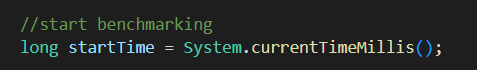
\includegraphics[width=0.8\columnwidth]{Figures/Week 2/Bench code Start.png}
        \caption{Screenshot of Java Benchmarking code at start of main}
        \label{fig:bench-code-start}
    \end{figure}
    
    \begin{figure}[H] 
        \centering
        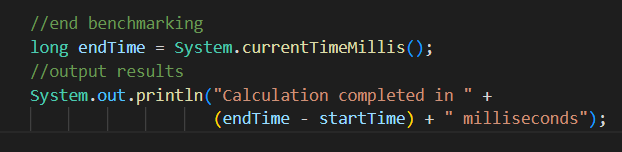
\includegraphics[width=0.8\columnwidth]{Figures/Week 2/Bench code end.png}
        \caption{Screenshot of Java Benchmarking code at end of main}
        \label{fig:bench-code-end}
    \end{figure}




    \begin{figure}[H] 
        \centering
        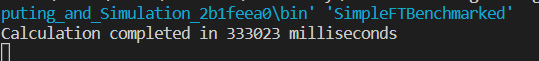
\includegraphics[width=0.8\columnwidth]{Figures/Week 2/SimpleFT Bench.png}
        \caption{Screenshot of the Console output from SimpleFT Benchmarking code}
        \label{fig:SimpleFT-Bench}
    \end{figure}
*
    \begin{figure}[H] 
        \centering
        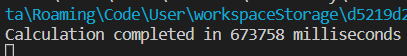
\includegraphics[width=0.8\columnwidth]{Figures/Week 2/SimpleFTFilters Bench.png}
        \caption{Screenshot of the output from SimpleFTFilters Benchmarking code}
        \label{fig:SimpleFTFilters-Bench}
    \end{figure}


    \begin{figure}[H] 
        \centering
        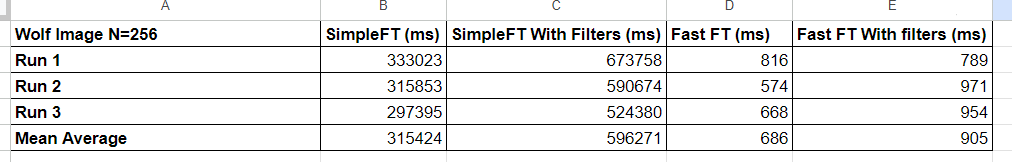
\includegraphics[width=1\columnwidth]{Figures/Week 2/Benchmarking results.png}
        \caption{Screenshot of the bench-marking results table}
        \label{fig:bench-results-table}
    \end{figure}
        

\section{Week 3 - CT Scanner}

This week two classes were supplied, DisplaySinogramFT.java outputted the SinogramFT as an image and Sinogram.java contained boilerplate code which includes the initial body slice model. It outputs the initial model and calculated sinogram before outputting a back-projected sinogram. The back-projected image contains very little detail, this is shown on the right side of \autoref{fig:W3-initial-output}.

The initial source model is the 'Shepp Logan Phantom' \textcite{6499235}, which is made of a series of ellipses representing different densities. The class performs an integral Radon Transform on the model densities to produce the Sinogram, the inversion of this transform will produce the final image. 


\begin{figure}[H] 
    \centering
    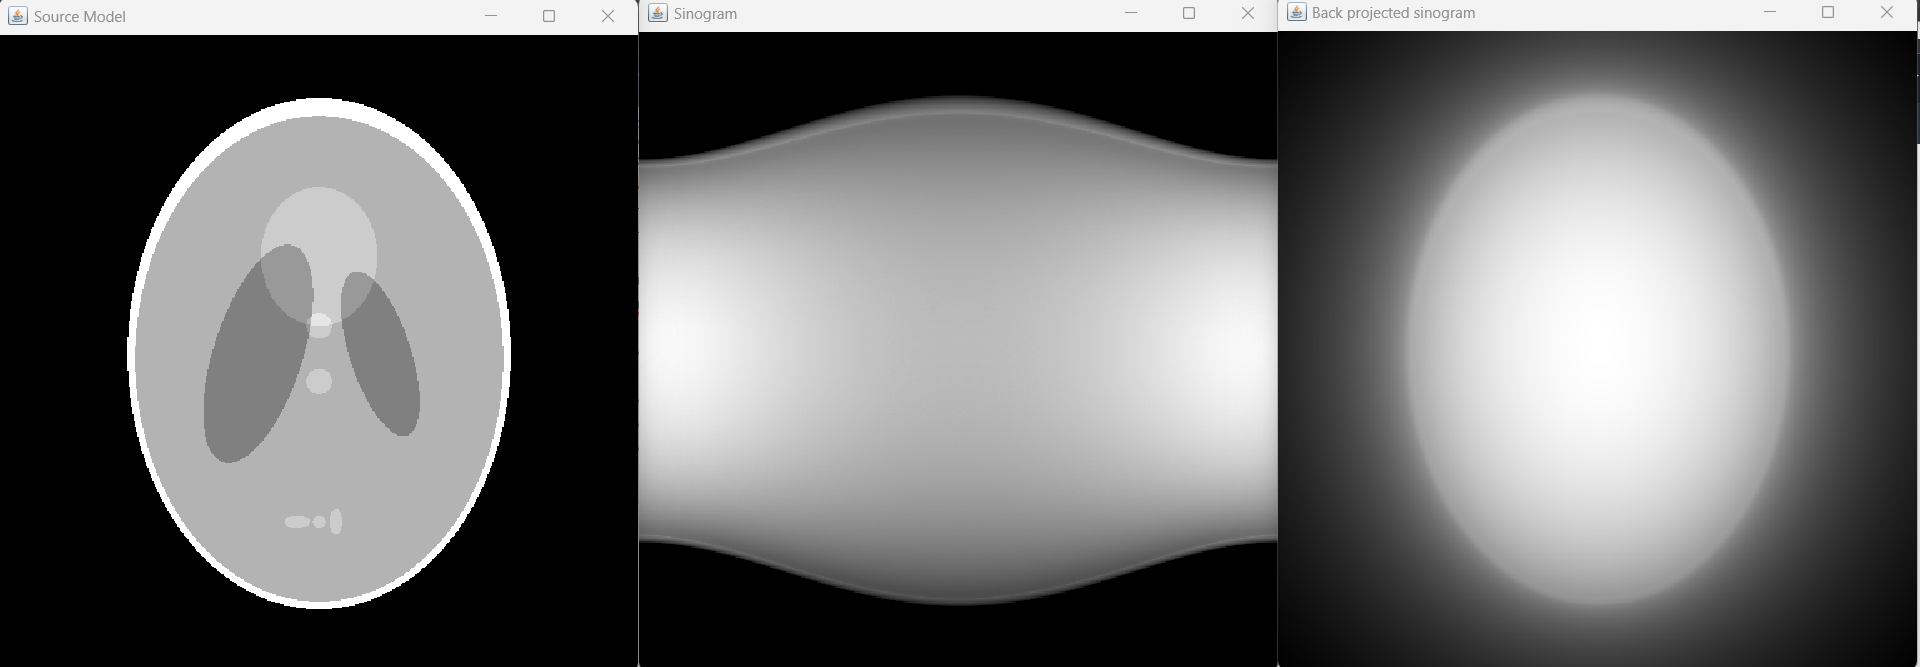
\includegraphics[width=0.9\columnwidth]{Figures/Week 3/initial-graphics.png}
    \caption{Screenshot of the graphical output of the initial Sinogram.java}
    \label{fig:W3-initial-output}
\end{figure}


\subsection{Applying an FFT}
Filtering the sinogram is required to make details more visible in the back-projected image. In order to perform filtering, a complex FFT is performed over \(\theta\) on the sinogram, the graphical output of this FFT is shown in \autoref{fig:W3-initial-FT}. Implementation code is shown in \autoref{fig:W3-initial-FT-code}.

\begin{figure}[H] 
    \centering
    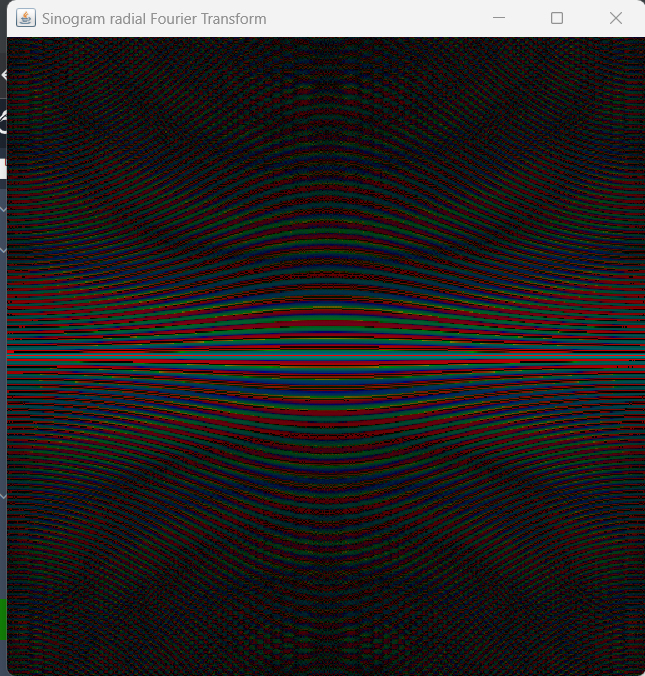
\includegraphics[width=0.9\columnwidth]{Figures/Week 3/initial-FFTpng.png}
    \caption{Screenshot of the graphical output of the initial Sinogram Fourier Transform}
    \label{fig:W3-initial-FT}
\end{figure}
\begin{figure}[H] 
    \centering
    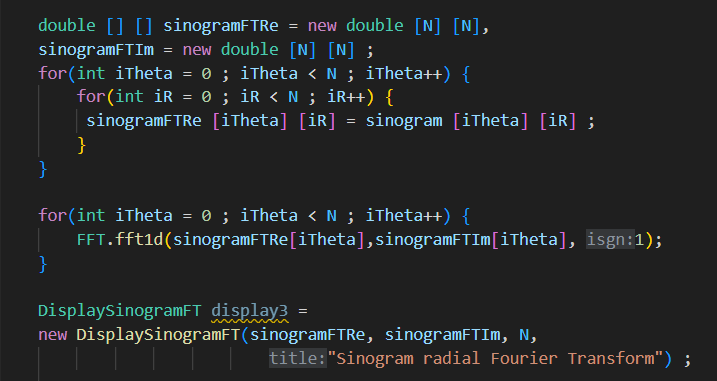
\includegraphics[width=0.49\columnwidth]{Figures/Week 3/initial-FFT-code.png}
    \caption{Screenshot of the code performing the Sinogram Fourier Transform}
    \label{fig:W3-initial-FT-code}
\end{figure}




\subsection{Applying a Simple Ramp Filter}
Next, the filter must be applied to the Fourier Transform data. A simple Ramp filter has been implemented. A ramp filter is a type of high-pass filter which reduces low frequencies to decrease blurring. The code performing this is shown in \autoref{fig:W3-ramp-code}. For each element, the code generates a $|K|$ value which is then multiplied to both the real and imaginary numerical components of the Fourier Transform.

The value of 'kSigned' is set to 'iK' if the value is $iK <= N/2$, otherwise, the value is set to $iK-N$.   
\begin{figure}[H] 
    \centering
    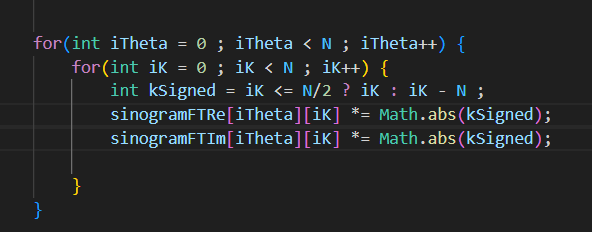
\includegraphics[width=0.9\columnwidth]{Figures/Week 3/ramp-filter-code.png}
    \caption{Screenshot of the code performing the Ramp filter}
    \label{fig:W3-ramp-code}
\end{figure}

The next step is to rebuild the Sinogram by performing an inverse Fourier Transform over \(\theta\), code is shown in \autoref{fig:W3-inverse-code}.

\begin{figure}[H] 
    \centering
    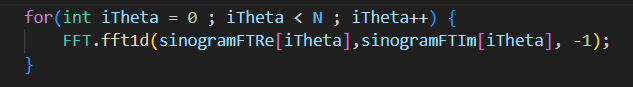
\includegraphics[width=0.9\columnwidth]{Figures/Week 3/inverse-FT.png}
    \caption{Screenshot of the code performing Inverse FT }
    \label{fig:W3-inverse-code}
\end{figure}

The filtered sinogram is shown in \autoref{fig:W3-filtered-sin}.
\begin{figure}[H] 
    \centering
    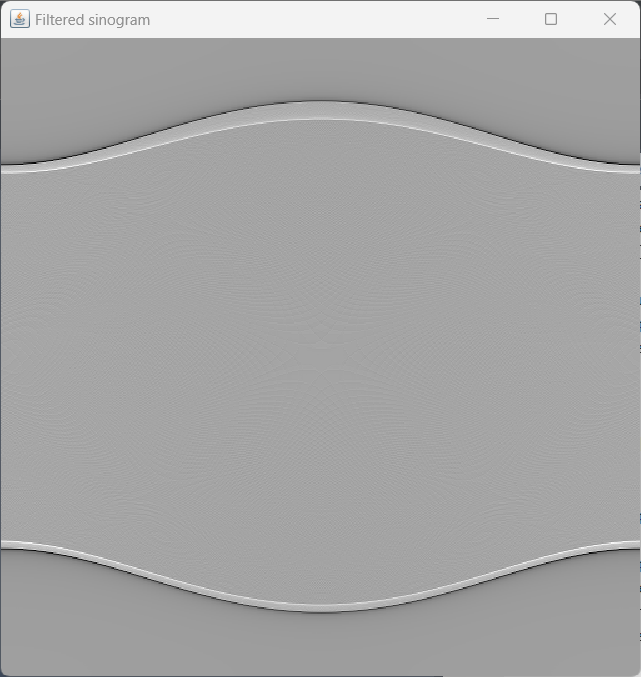
\includegraphics[width=0.9\columnwidth]{Figures/Week 3/filtered-sinorgram.png}
    \caption{Screenshot of the graphical output for the filtered sinogram}
    \label{fig:W3-filtered-sin}
\end{figure}

To output the filtered back-projected image, a back-projection operation is performed on the sinogram before the values are normalised. The new image is then drawn. This is shown in \autoref{fig:W3-filtered-back-image}. More detail is visible in the back-projected image, however, a lot of noise has been introduced. To reduce this noise, further filtering is required.
    
\begin{figure}[H] 
    \centering
    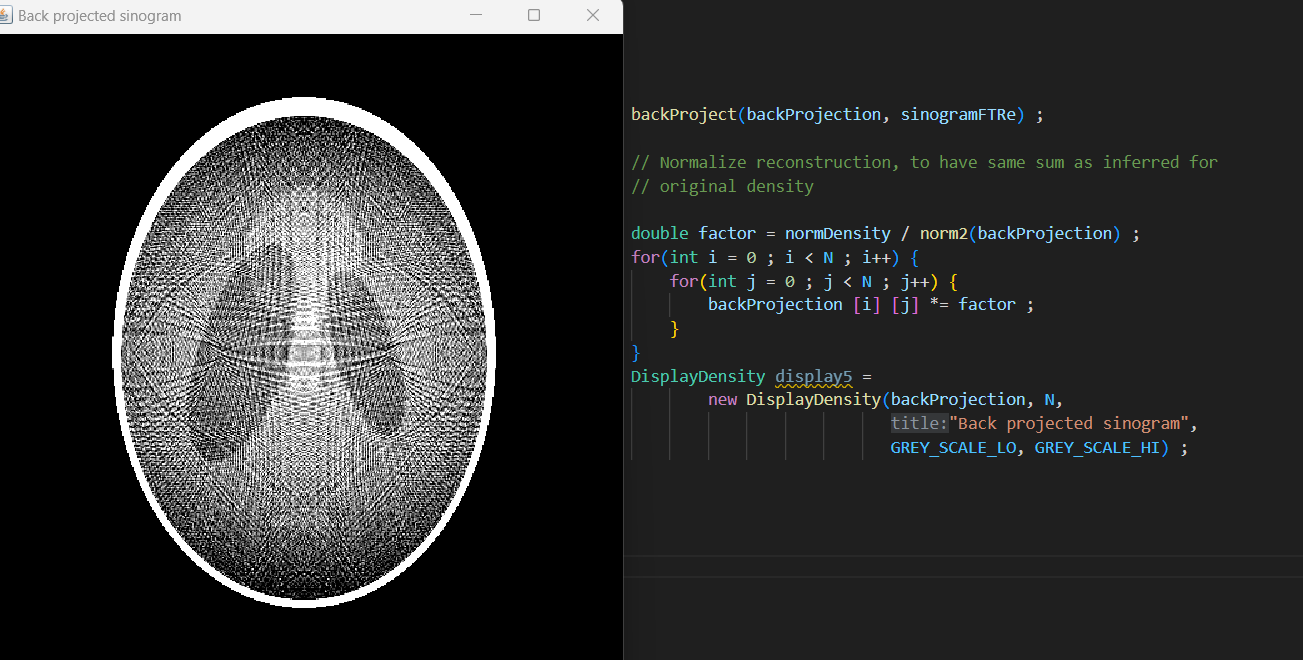
\includegraphics[width=1\columnwidth]{Figures/Week 3/filtered-back-projection.png}
    \caption{Screenshot the filtered back-projected sinogram}
    \label{fig:W3-filtered-back-image}
\end{figure}


\subsection{Applying a Ramp Filter with Cutoffs}
The previous filter was altered to make use of a cutoff value, an integer variable 'CUTOFF' was created. This stores the value of: '$N / Value$'. If the '$|K|$' value is greater than this CutOff, the Fourier Component is set to '0'. The code for this implementation is shown in \autoref{fig:W3-filter-with-cutoff-code}.

\begin{figure}[H] 
    \centering
    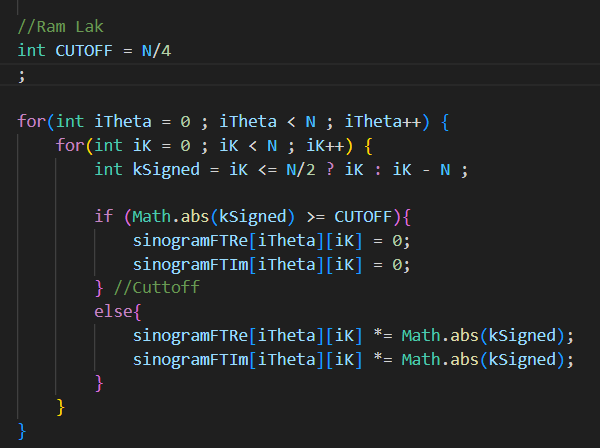
\includegraphics[width=1\columnwidth]{Figures/Week 3/Filter-with-cuttoff-code.png}
    \caption{Screenshot of the Java code performing filtering with cutoff value}
    \label{fig:W3-filter-with-cutoff-code}
\end{figure}


The program was run with $N/4$ and $N/16$, the back-projected images do have slightly reduced noise. \autoref{fig:W3-many-filters} shows the back-projected images made using a Ramp filter with no CUTOFF (left), with CUTOFF=N/4 (centre) and CUTOFF=N/16 (right).  



\begin{figure}[H] 
    \centering
    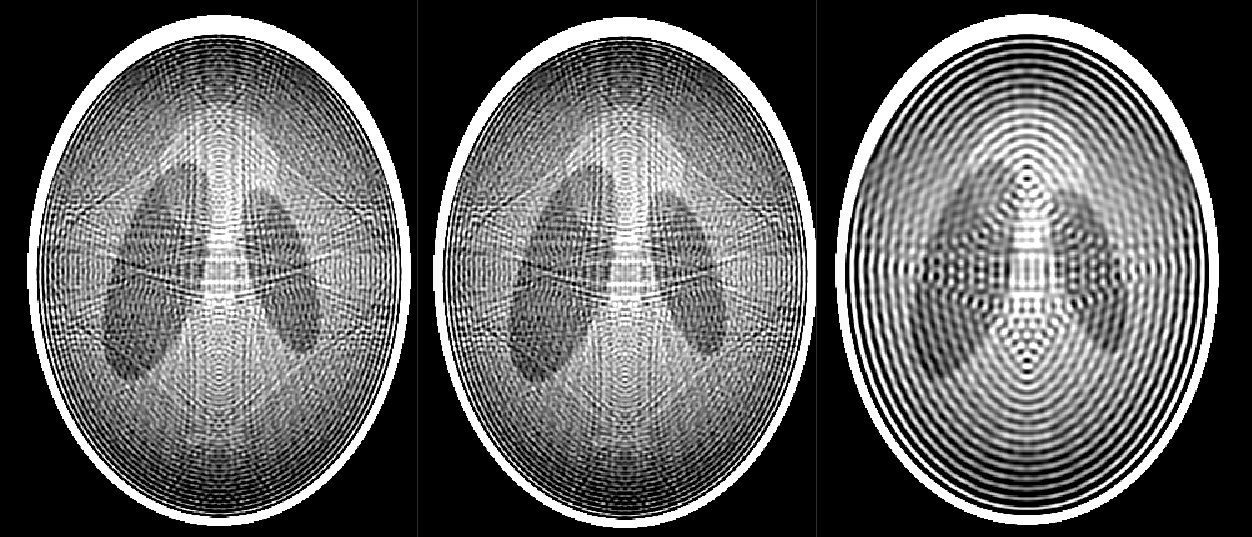
\includegraphics[width=1\columnwidth]{Figures/Week 3/filtered-images-ramp-N-4-N-16.png}
    \caption{Screenshot of back project images with filters applied}
    \label{fig:W3-many-filters}
\end{figure}


\newpage
\subsection{Applying Low Pass Cosine Filter}

Next, a low-pass Cosine Filter was applied. The filter takes a similar approach to the previous high pass filter but applies: $|K|$  $cos(\pi K /(2  *  CUTOFF))$.

Implementation is shown in \autoref{fig:W3-cos-filter-code}. 

\begin{figure}[H] 
    \centering
    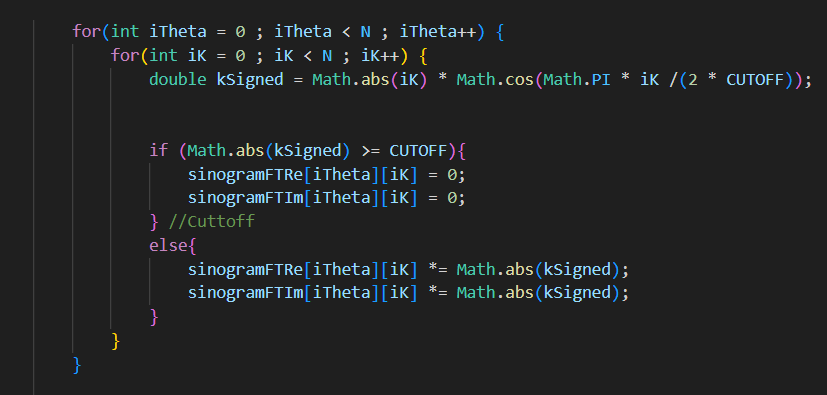
\includegraphics[width=1\columnwidth]{Figures/Week 3/filter-cos-codfe.png}
    \caption{Screenshot of the cosine filter code}
    \label{fig:W3-cos-filter-code}
\end{figure}

\autoref{fig:W3-cos-filter-image} shows the image when CUTOFF=$N/4$. The image has little noise removed,
\autoref{fig:W3-cos-filter-image-n-8} shows the image when CUTOFF=$N/8$, the image is now missing a lot of detail compared to the results of the standard ramp filter. 
\begin{figure}[H] 
    \centering
    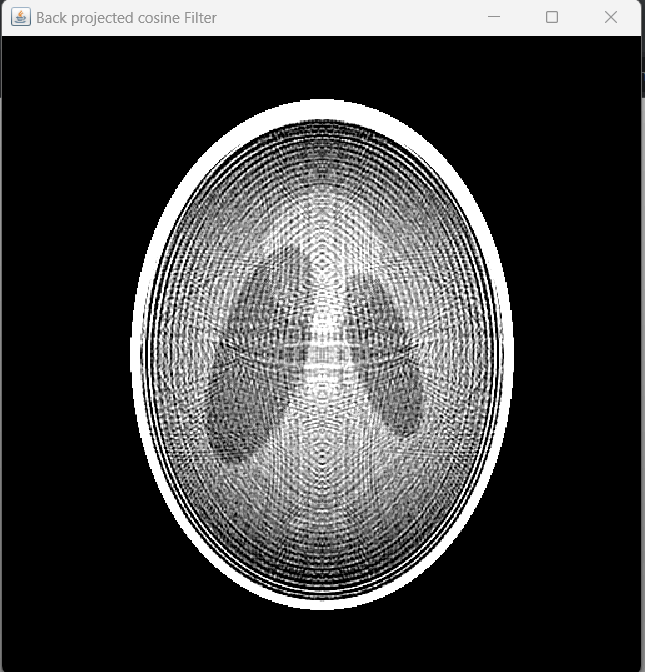
\includegraphics[width=0.49\columnwidth]{Figures/Week 3/filter-cos-image.png}
    \caption{Screenshot of the cosine filter image Cutoff=N/4}
    \label{fig:W3-cos-filter-image}
\end{figure}
\begin{figure}[H] 
    \centering
    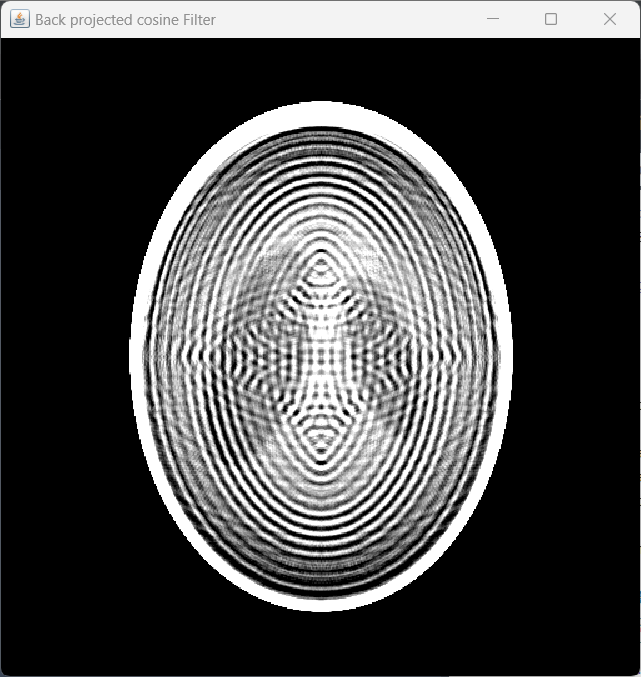
\includegraphics[width=0.49\columnwidth]{Figures/Week 3/filter-cos-image-N-8.png}
    \caption{Screenshot of the cosine filter image Cutoff=N/8}
    \label{fig:W3-cos-filter-image-n-8}
\end{figure}


\section{Week 4}
\section{Week 5}
\section{Week 6}
\section{Week 7}
\section{Week 8}
\section{Week 9}
\section{Week 10}
\section{Week 11}
